\chapter[Modelos basados en partes ]{Modelos para detección de objetos basados en partes discriminadamente entrenados }\label{ch:framework}
introducción...

\section{Marco de desarrollo}
Para realizar el procesamiento del conjunto de datos se utiliza un marco de desarrollo creado por Felzenszwalb et al.~\cite{Felzenszwalb2010}, el cual nos permitirá generar los modelos para el reconocimiento de los objetos que analizaremos. Este marco está basado en el conjunto de imágenes de PASCAL~\cite{Everingham2010}.

\subsection{Definición de datos}
La definición de los datos es una etapa muy importante en este tipo de estudios, ya que es en esta etapa donde se seleccionan los datos a ser procesados, utilizando diversas especificaciones y formas de representar estos datos de entrada. Para el estudio realizado por Felzenszwalb et al.~\cite{Felzenszwalb2010}, se utiliza la base de datos PASCAL~\cite{Everingham2010}, la cual provee un conjunto de imágenes y anotaciones, más adelante explicado.

<<<<<<< HEAD
Se necesita detallar información específica de cada imagen, por lo que es necesario crear un archivo XML, con el mismo nombre de la imagen, que contenga la información necesaria para realizar el procesamiento, esto es llamado, anotación. La anotación especifica la clase de la muestra, la ruta del archivo; de dónde se obtuvo la imagen; entre otros atributos necesarios de las imágenes de entrenamiento. Lo más importante de estas anotaciones es que contiene la o las \textbf{regiones} de interés, dependiendo de cuántos objetos contenga la imagen. Una región, está representada por cuatro pixeles, los que a su vez, representan los vértices de una diagonal en un plano cartesiano, dónde su origen se encuentra ubicado en la esquina superior izquierda de la imagen. Es importante mencionar, que tanto el eje $x$ como el eje $y$, son positivos, por lo que cada pixel representa la distancia al origen, este proceso se puede ver en la Figura~\ref{fig:anota}
=======
Se necesita detallar información específica de cada imagen, por lo que es necesario crear un archivo XML, con el mismo nombre de la imagen, que contenga la información necesaria para realizar el procesamiento, esto es llamado, anotación. La anotación especifica la clase de la muestra, la ruta del archivo; de dónde se obtuvo la imagen; entre otros atributos necesarios de las imágenes de entrenamiento. Lo más importante de estas anotaciones es que contiene la o las \textbf{regiones} de interés, dependiendo de cuántos objetos contenga la imagen. Una región, está representada por cuatro pixeles, los que a su vez, representan los vértices de una diagonal en un plano cartesiano, dónde su origen se encuentra ubicado en la esquina superior izquierda de la imagen. Es importante mencionar, que tanto el eje $x$ como el eje $y$, son positivos, por lo que cada pixel representa la distancia al origen, este proceso se puede ver en la Figura~\ref{fig:anota}.
>>>>>>> 3bab0826051589fef1f771e88493714c764b5522

\begin{figure}[tb]
  \centering
   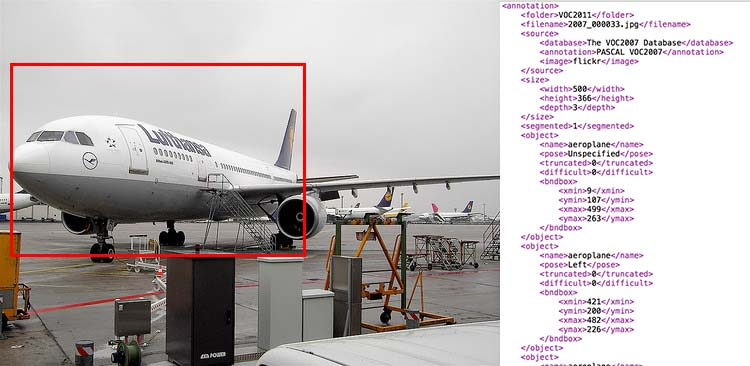
\includegraphics[width=0.4\textwidth]{Figuras/plain-1.jpg}
   \caption{Esquema de anotación}
   \label{fig:anota}
\end{figure}

\subsection{Preprocesamiento}
Una vez creadas todas las anotaciones, se puede iniciar el proceso de creación del modelo. En primera instancia, se separan los conjuntos de datos en tres partes: Datos positivos, es decir, aquellos donde se encuentra el objeto; Datos negativos, aquellas imágenes donde no hay presencia de la clase buscada y finalmente en datos negativos difíciles, el que contiene imágenes donde hay objetos muy parecidos a simple vista. La estructura del modelo será analizada con mayor detalle en la sección~\ref{sec:model}.

La cantidad de muestras ó tipos de imágenes, pueden variar influyendo directamente en el resultado, afectando la efectividad que se haya obtenido en el paso anterior, por lo que es muy importante encontrar y preprocesar un buen conjunto de entrenamiento en una etapa temprana.


\section{Modelo de entrenamiento}
\label{sec:model}
Nuestro modelo estará basado por lo presentado en el estado del arte, específicamente, lo realizado por Felzenszwalb et al.~\cite{Felzenszwalb2010}. Esto nos permitirá crear un modelo el cual nos ayudará a clasificar de mejor manera las clases que en este trabajo estamos buscando clasificar. A continuación detallaremos la estructura del marco de desarrollo tratando de explicar y analizar los puntos más importantes de éste.

Según explica Felzenszwalb et al.~\cite{Felzenszwalb2010}, todos los modelos generados por el marco involucran filtros lineales, los cuales son aplicados en mapas de características densos. De estos mapas se extraen las características más representativas y se crea un vector de características que describe la porción de la imagen que se está observando. A demás, estas características son descritas mediante HOG el cual fue creado por Dalal and Triggs~\cite{Dalal2005}, aun así el marco de desarrollo es independiente del tipo de extractor de características que se utilice.

Los filtros son definidos por un arreglo de \textit{d} dimensiones de vectores de peso. Felzenszwalb et al.~\cite{Felzenszwalb2010}, define los \textit{scores} en distintas posiciones y escalas de la imagen observada, esto se realiza obteniendo las características de la pirámide, esta pirámide, consiste en hacer varias corridas de la misma imagen con distintas resoluciones, donde en cada nivel de resolución se extraen las características más representativas. En la práctica, los niveles de la pirámide son definidos por $\lambda$. Se usa $\lambda = 5$ para entrenar y $\lambda = 10$ para probar el modelo.

\subsection{Deformable Part Models}
\label{subsec:dpm}
Este modelo está definido por un filtro raíz que aproximadamente cubre un objeto completo y por filtros de alta resolución que cubren partes más pequeñas del objeto. El filtro raíz define la ventana principal para la detección. Los filtros por cada parte del objeto son ubicados $\lambda$ niveles abajo en la pirámide. Las característica en ese nivel son procesados al doble de resolución de las características sobre el filtro de la raíz.
Con estos pasos, Felzenszwalb et al.~\cite{Felzenszwalb2010}~\cite{Felzenszwalb2013}, a encontrado que usando funciones de mayor resolución para definir filtros de partes, es fundamental para obtener un rendimiento más mayor en la tarea de reconocimiento.

\subsection{Matching}
\label{subsec:matching}
Para detectar un objeto en una imagen, se calcula un score general sobre la raíz de la imagen de acuerdo al mejor posicionamiento de las partes, 
\begin{equation}
	score(p_{0}) = \max_{p_{1}, ..., p_{n}} score(p_{0}, ..., p_{n}).
\end{equation} 
Una detección es definida por un alto score de las posiciones de la raíz, mientras que las posiciones de las partes con alto score definen la hipótesis de un objeto completo.

Mediante la definición de una score global para cada posición de la raíz se puede detectar varias instancias de un objeto.

\subsection{Mixture Models}
\label{subsec:mm}